\documentclass{article}
\usepackage{geometry}
\geometry{a4paper,scale=0.9}
\usepackage[utf8]{inputenc}

\usepackage{amssymb}
\usepackage{graphicx}

\title{Rapport TP4}

\author{Rosine Rolande Simo Tegninko, 20183729\\
Yu Deng, 20151659}

\date{}

\begin{document}

\maketitle

\section*{TESTS BOITE NOIRE}\\

Dans ce test, il y a deux conditions de test requises :\\

$\cdot$ Convertir des montants uniquement entre les devises suivantes : USD, CAD, GBP, EUR, CHF, INR, AUD.

$\cdot$ Seulement accepter des montants entre [0, 10000].\\

\textbf{Pour le type de devise}\\

Dans le code, il existe un moyen de construire des objets de type CurrencyConversion. Cela générera des objets contenant plusieurs devises, qui peuvent répondre à nos exigences de test. De plus, j'ai choisi de réutiliser le même code pour plus de commodité. La structure de base du test est la suivante. Déterminez si chaque cas de test réussit en jugeant le résultat de l'exécution de la couverture ou de l'exception levée.\\
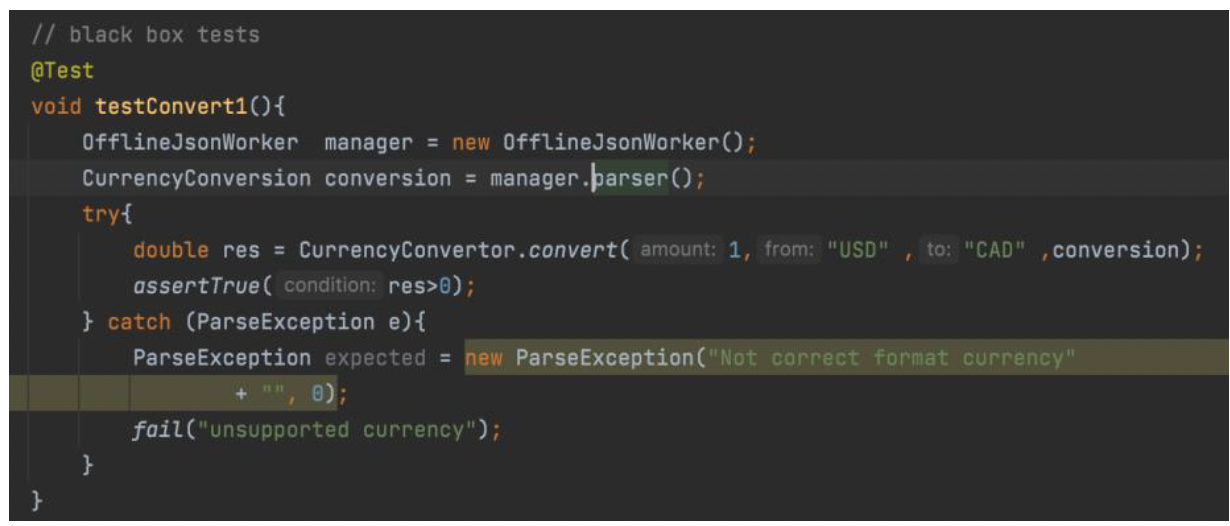
\includegraphics[scale=0.5]{G1.png}\\

Dans le cas de test 1, j'ai sélectionné USD et CAD pour la conversion. Les deux sont des types de devises qui peuvent être convertis. Cette affaire peut passer sans problème. Ensuite, j'autoriserai la conversion de sept devises pour passer le test par paires.\\
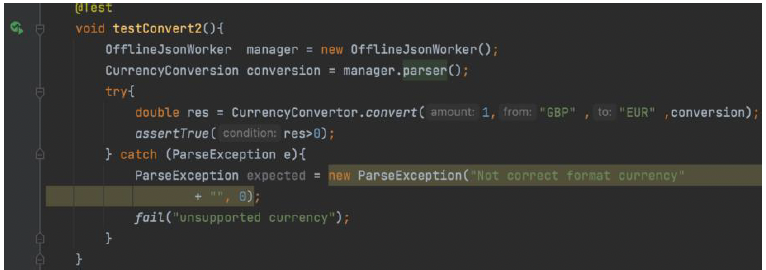
\includegraphics[scale=0.7]{G2.png}\\

Lorsque j'utilise AUD et FJD qui ne devraient pas être pris en charge pour la conversion, je trouve que l'assertion de résultat renvoie toujours le résultat normalement et j'utilise fail() pour générer des informations d'erreur, ce qui indique que convert() lui-même ne contraint pas le type de devise nous exigeons.\\
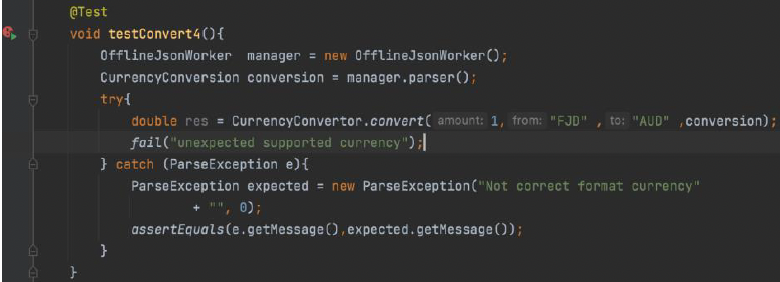
\includegraphics[scale=0.7]{G3.png}\\

\textbf{Pour plage numérique}\\

Pour le test d'intervalle numérique, j'ai sélectionné le point final de l'intervalle, dans l'intervalle et hors de l'intervalle.\\
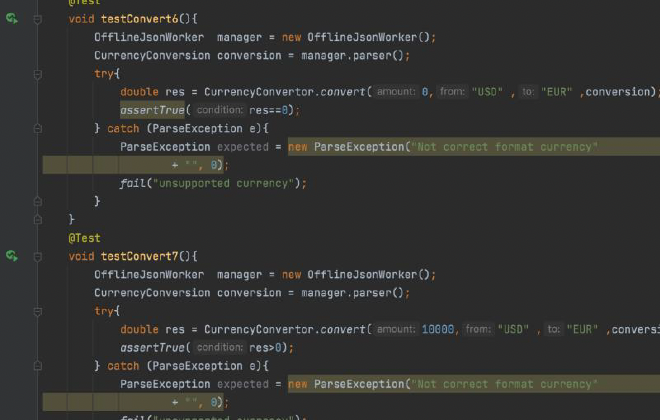
\includegraphics[scale=0.6]{G4.png} 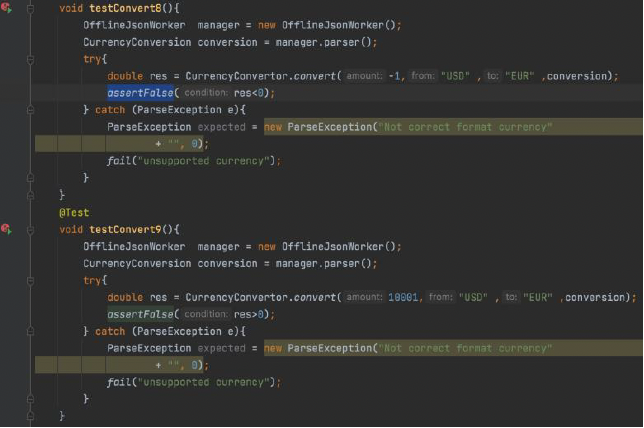
\includegraphics[scale=0.65]{G5.png}\\

Les valeurs dans l'intervalle et à la fin de l'intervalle ont passé avec succès la vérification des résultats, mais lorsque je suis allé à -1 et 10001, j'ai toujours renvoyé res normalement. En fait, ce n'est pas autorisé. Par conséquent, assertFalse échoue ici. De toute évidence, la fonction de conversion n'impose pas la limite numérique requise sur la valeur "amount".\\



\end{document}
